\documentclass{article}
\usepackage{blindtext}
\usepackage[utf8]{inputenc}
\usepackage{amsmath,bm}
\usepackage{amstext}
\usepackage{amsfonts}
\usepackage[UTF8]{ctex}
\usepackage{amsmath}
\usepackage{changepage}
\usepackage{graphicx} 
\usepackage{subfigure}
\usepackage{color,soul}
\usepackage[utf8]{inputenc}
\usepackage[english]{babel} 
\usepackage{tikz}
\usetikzlibrary{positioning}
\title{Introduction to Machine Learning\\Homework 1}
\author{吴紫航 171860659}
\date{} 
\begin{document}
	\maketitle
	\numberwithin{equation}{section}	
	\section{[20pts] Basic review of probability}
	The probability distribution of random variable $X$ follows:\\
	\begin{equation}
	f_X(x)=\begin{cases}
	\frac{1}{2} & 0<x<1;\\
	\frac{1}{6} & 2<x<5;\\
	0 & \text{otherwise}.
	\end{cases}
	\end{equation} 
	(1) [5pts] Please give the cumulative distribution function $F_X(x)$ for X;\\
解: \\
\indent当 $x<0$, $F_X(x)=0$;\\
\indent当$0\leq x<1, F_X(x)=\int_{-\infty}^{x}f_X(x)dx=\int_{0}^{x}\frac{1}{2}dx=\frac{x}{2};$\\
\indent当$1\leq x<2$, $F_X(x)=\frac{1}{2}$; \\
\indent当$2\leq x<5, F_X(x)=\frac{1}{2}+\int_{2}^{x}\frac{1}{6}dx=\frac{1}{2}+\frac{x}{6}-\frac{1}{3}=\frac{x+1}{6}; $ \\
\indent当$x\geq5,F_X(x)=1; $\\\\
\indent 因此,随机变量$X$的分布函数$F_X(x)$为
		\begin{equation}
		F_X(x)=\begin{cases}
			0&x<0;\\
			\frac{x}{2}&0\leq x<1;\\
			\frac{1}{2}&1\leq x<2;\\
			\frac{x+1}{6}&2\leq x<5;\\
			1&x\geq5.\\
		\end{cases}
		\end{equation}
\\\\
	(2) [5pts] Define random variable $Y$ as $Y=1/(X^2)$, please give the probability density function $f_Y(y)$ for $Y$;\\
解:\\
\indent当$y\leq0,$ $F_Y(y)=0$;\\
\indent当$y>0,$ $F_Y(y)=P(Y\leq y)=P(\frac{1}{X^2}\leq y)$\\
\indent$=P(X\geq \frac{1}{\sqrt y})+P(X\leq -\frac{1}{\sqrt y})=1-P(X< \frac{1}{\sqrt y})+P(X\leq -\frac{1}{\sqrt y})$\\
\indent$=1-F_X(\frac{1}{\sqrt y})+F_X(-\frac{1}{\sqrt y})=1-F_X(\frac{1}{\sqrt y})$;\\\indent进一步细分\\
\indent当$y>1,$ $F_Y(y)=1-\frac{1}{2\sqrt y}$;\\
\indent当$\frac{1}{4}<y\leq1,$ $F_Y(y)=1-\frac{1}{2}=\frac{1}{2}$;\\
\indent当$\frac{1}{25}<y\leq \frac{1}{4}$, $F_Y(y)=1-\frac{1}{6}(\frac{1}{\sqrt y}+1)=\frac{1}{6}(5-\frac{1}{\sqrt y}) $;\\
\indent当$0<y\leq \frac{1}{25}$, $F_Y(y)=0$;\\
\indent经过求导得, 随机变量y的概率密度函数$f_Y(y)$为\\
		\begin{equation}
		f_Y(y)=\begin{cases}
			\frac{1}{12\sqrt {y^3}}&\frac{1}{25}<y\leq \frac{1}{4};\\
			\frac{1}{4\sqrt{y^3}}&y>1;\\
			0 & \text{otherwise}.
		\end{cases}
		\end{equation}
\\
	(3) [10pts] For some random non-negative random variable Z, please prove the following two formulations are equivalent:\\
	\begin{equation}
	\mathbb{E}[Z]=\int^\infty_{z=0} z f(z)\mathrm{d}z,
	\end{equation}
	\begin{equation}
	\mathbb{E}[Z]=\int^\infty_{z=0} \mathrm{Pr}[Z\geq z]\mathrm{d}z,
	\end{equation}
	Meantime, please calculate the expectation of random variable $X$ and $Y$ by these two expectation formulations to verify your proof.\\
解:\\
\indent$\int^\infty_{z=0} \mathrm{Pr}[Z\geq z]\mathrm{d}z=\int_{z=0}^\infty \int_{z}^\infty f(t)dtdz=\int_{z=0}^\infty \int_{0}^\infty f(t)one(t)dtdz$\\
\indent ps: $one(t)=1$, 当$t\geq z$; $one(t)=0$, 当$t<z$.\\
\indent则由fubini定理, $\int^\infty_{z=0} \mathrm{Pr}[Z\geq z]\mathrm{d}z=\int_{z=0}^\infty f(t)\int_{0}^\infty one(z)dzdt=\int_{z=0}^\infty f(t)tdt$\\
\indent ps: $one(z)=1$, 当$z\leq t$; $one(z)=0$, 当$z>t.thus,\int_{0}^\infty one(z)dz=t$\\
\indent 因此, 两种数学期望的表达形式是等价的.\\
\indent 接下来验证X和Y的分布满足这两种数学期望相等价的结论.\\
\indent 对于$X$, $\mathbb{E}[X]=\int_{x=0}^\infty xf(x)dx=\int_{0}^{1}\frac{x}{2}dx+\int_{2}^{5}\frac{x}{6}dx=2$;\\
\indent 同时$\mathbb{E}[X]=\int^\infty_{x=0} \mathrm{Pr}[X\geq x]\mathrm{d}x=\int^{1}_{0}(1-\frac{x}{2})dx+\int^{2}_{1}\frac{1}{2}dx+\int_{2}^{5}\frac{5-x}{6}dx$\\
\indent$=\frac{3}{4}+\frac{1}{2}+\frac{3}{4}=2$. 因此$X$的分布满足结论, 数学期望为 $\mathbb{E}[X]=2$\\\\
\indent 对于$Y$, $\mathbb{E}[Y]=\int_{y=0}^\infty yf(y)dy=\int_{\frac{1}{25}}^{\frac{1}{4}}\frac{y}{12\sqrt{y^3}}dy+\int_{1}^{\infty}\frac{y}{4\sqrt{y^3}}dy=\infty$;\\
\indent 同时$\mathbb{E}[Y]=\int^\infty_{y=0} \mathrm{Pr}[Y\geq y]\mathrm{d}y=\int^{\frac{1}{25}}_{0}dy+\int^{\frac{1}{4}}_{\frac{1}{25}}\frac{1}{6}(1+\frac{1}{\sqrt y})dy+\int_{\frac{1}{4}}^{1}\frac{1}{2}dy$\\
\indent$+\int_{1}^{\infty}\frac{1}{2\sqrt{y}}dy= \infty$. \\
\indent因此$Y$的分布满足结论, 数学期望为 $\mathbb{E}[Y]=\infty$.\\
	
	\section{[15pts] Probability Transition}

	\noindent(1) [5pts] Suppose P(rain today) = 0.30, P(rain tomorrow) = 0.60,
	P(rain today and tomorrow) = 0.25. Given that it rains today, what
	is the probability it will rain tomorrow?\\
解:\\
\indent 设$A$事件\{今天下雨\}; $B$事件\{明天下雨\}.\\
\indent 则由题干得, $P(A)=0.3,P(B)=0.6,P(AB)=0.25$\\
\indent 则已知今天下雨的条件下,明天下雨的概率为$P(B|A)=\frac{P(AB)}{P(A)}=\frac{5}{6}$\\
\indent 因此,已知今天下雨的条件下,明天下雨的概率是$\frac{5}{6}$.\\
\\
	(2) [5pts] Give a formula for $P(G | \neg H)$ in terms of $P(G)$,
	$P(H)$ and $P(G \wedge H)$ only.  Here $H$ and $G$ are boolean random variables.\\
解:\\
\indent$P(G|\mathop{H}\limits^{\neg})=\frac{P(G\wedge \mathop{H}\limits^{\neg})}{1-P(H)}=\frac{P(G)-P(G\wedge H)}{1-P(H)}$.\\\\\\
	(3) [5pts] A box contains {\it w} white balls and {\it b} black
	balls. A ball is chosen at random. The ball is then replaced,
	along with {\it d} more balls of the same color (as the chosen
	ball). Then another ball is drawn at random from the box. Show
	that the probability that the second ball is white does not depend
	on {\it d}.  \\\\
解:\\
\indent 设事件$A_1$\{第一次拿白球\},事件$A_2$\{第一次拿黑球\},\\
\indent事件$B$\{第二次拿白球\}\\
\indent 则$P(B)=P(A_1)P(B|A_1)+P(A_2)P(B|A_2)$\\
\indent$=\frac{w}{w+b}\times\frac{w+d-1}{w+b+d-1}+\frac{b}{w+b}\times\frac{w}{w+b+d-1}=\frac{w}{w+b}$\\
\indent显然结果和d无关
	\section{[20pts] Basic review of Linear Algebra}
	Let $x = (\sqrt{3}, 1)^{\top}$ and $y = (1, \sqrt{3})^{\top}$ be two vectors,\\\\
	(1) [5pts] What is the value of $x_{\perp}$ where $x_{\perp}$ indicates the projection of $x$ onto $y$. \\
解:\\
\indent $x\cdot y=x^{\top}y=2\sqrt{3}$, $|y|=\sqrt{1+3}=2$\\
\indent 因此$x$在$y$上的投影大小为$||x_{\perp}||=\frac{2\sqrt3}{2}=\sqrt{3},$ 投影为$x_{\perp}=(\frac{\sqrt3}{2},\frac{3}{2})^{\top}$
\\
	(2) [5pts] Prove that $y \perp (x - x_{\perp})$.\\
解:\\
\indent $x-x_{\perp}=(\sqrt3,1)^{\top}-(\frac{\sqrt3}{2},\frac{3}{2})^{\top}=(\frac{\sqrt3}{2},-\frac{1}{2})^{\top}$\\
\indent 则$y^{\top}(x-x_\perp)=(1,\sqrt3)\cdot(\frac{\sqrt3}{2},-\frac{1}{2})^{\top}=0$\\
\indent因此 $y\perp(x-x_\perp).$\\
\\
	(3) [10pts] Prove that for any $\lambda \in \mathbb{R}$, $\lvert| x - x_{\perp}\rvert| \leq \lvert| x - \lambda y \rvert|$ \\
解:\\
\indent由$\lvert|x-x_\perp\rvert|=\sqrt{\frac{3}{4}+\frac{1}{4}}=1$\\
\indent又$\lvert|x-\lambda y\rvert|=\sqrt{(\sqrt3-\lambda)^2+(1-\sqrt3\lambda)^2}=\sqrt{4\lambda^2-4\sqrt3\lambda+4}$\\
\indent$=2\sqrt{(\lambda-\frac{\sqrt3}{2})^2+\frac{1}{4}}\geq 2\sqrt{\frac{1}{4}}=1$\\
\indent故$\lvert| x - x_{\perp}\rvert| \leq \lvert| x - \lambda y \rvert|,$ 当且仅当$\lambda=\frac{\sqrt3}{2}时,$ 取等号 \\
	
	\section{[20pts] Hypothesis Testing}
	A coin was tossed for $50$ times and it got $35$ heads, please determine that \emph{if the coin is biased for heads} with $\alpha = 0.05$.\\
解:\\
\indent设$p$为硬币正面朝上的概率,则该问题可归结为如下假设检验问题:\\
\indent$H_0:E_X=0.5,$ $H_1:E_X> 0.5$,\\
\indent设$x$为正面朝上的次数,若原假设成立,则$x\sim(50,0.5)$.\\
\indent样本较大,由中心极限定理,近似为正态分布计算.\\
\indent统计量取$u=\frac{x-50\times0.5}{\sqrt{50\times0.5\times(1-0.5)}}$,\\
\indent即近似认为$u\sim N(0,1)$, 故检验拒绝域为$W=\{u>u_{1-\alpha}\}$\\
\indent$=\{u>1.645\}$\\
\indent检验的$p$值近似计算为:\\
\indent$p=P\{x\geq35\}=P\{u\geq{\frac{35-25}{\sqrt{\frac{25}{2}}}}\}=P\{u\geq2\sqrt2\}=0.0023<0.5$\\
\indent结果落在拒绝域内,因此拒绝原假设,认为硬币更倾向于正面朝上.
\\\\	
	\section{[25pts] Performance Measures}
	We have a set of samples that we wish to classify in one of two classes and a ground truth class of each sample (denoted as 0 and 1). For each example a classifier gives us a score (score closer to 0 means class 0, score closer to 1 means class 1). Below are the results of two classifiers ($C_1$ and $C_2$) for 8 samples,their ground truth values ($y$) and the score values for both classifiers ($y_{C_1}$ and $y_{C_2}$).
	\begin{table}[htbp]
		\centering
		\begin{tabular}{c|cccccccc}
			\hline
			$y$ & 1 & 0 & 1 & 1 & 1 & 0 & 0 & 0\\
			\hline
			$y_{C_1}$ & 0.6 & 0.31 & 0.58 & 0.22 & 0.4 & 0.51 & 0.2 & 0.33\\
			\hline
			$y_{C_2}$ & 0.04 & 0.1 & 0.68 & 0.24 & 0.32 & 0.12 & 0.8 & 0.51\\
			\hline
		\end{tabular}
	\end{table}

	\noindent{(1) [10pts] For the example above calculate and draw the ROC curves for classifier $C_1$ and $C_2$. Also calculate the area under the curve (AUC) for both classifiers.}\\\\
解:\\
\indent(a)先确定C1的ROC曲线和AUC大小\\
\indent排序后C1表格为
\begin{table}[htbp]
		\centering
		\begin{tabular}{c|cccccccc}
			\hline
			$y$ & 0 & 1 & 0 & 0 & 1 & 0 & 1 & 1\\
			\hline
			$y_{C_1}$ & 0.2 & 0.22 & 0.31 & 0.33 & 0.4 & 0.51 & 0.58 & 0.6\\
			\hline
		\end{tabular}
	\end{table}
\\
\indent由此得到ROC曲线上的点为$(0,0)$、$(0,\frac{1}{4})$、$(0,\frac{1}{2})$、$(\frac{1}{4},\frac{1}{2})$、$(\frac{1}{4},\frac{3}{4})$、\\
\indent$(\frac{1}{2},\frac{3}{4})$、$(\frac{3}{4},\frac{3}{4})$、$(\frac{3}{4},1)$、$(1,1)$\\
\indent因此ROC曲线图为
\begin{figure}[htb]   \center{\includegraphics[width=12cm]  {C1ROC.png}}      \end{figure} \\
\indent 则$AUC_{C1}=\frac{1}{4}\times\frac{1}{2}+\frac{1}{2}\times\frac{3}{4}+\frac{1}{4}\times1=\frac{3}{4}$
\\\\\\
\indent(b)再确定C2的ROC曲线和AUC大小\\
\indent排序后C2表格为
\begin{table}[htbp]
		\centering
		\begin{tabular}{c|cccccccc}
			\hline
			$y$ & 1 & 0 & 0 & 1 & 1 & 0 & 1 & 0\\
			\hline
			$y_{C_2}$ & 0.04 & 0.1 & 0.12 & 0.24 & 0.32 & 0.51 & 0.68 & 0.8\\
			\hline
		\end{tabular}
	\end{table}
\\
\indent由此得到ROC曲线上的点为$(0,0)$、$(\frac{1}{4},0)$、$(\frac{1}{4},\frac{1}{4})$、$(\frac{1}{2},\frac{1}{4})$、$(\frac{1}{2},\frac{1}{2})$、\\
\indent$(\frac{1}{2},\frac{3}{4})$、$(\frac{3}{4},\frac{3}{4})$、$(1,\frac{3}{4})$、$(1,1)$\\
\indent因此ROC曲线图为
\begin{figure}[htb]   \center{\includegraphics[width=12cm]  {C2ROC.png}}      \end{figure} \\
\indent $AUC_{C2}=\frac{1}{4}\times\frac{1}{4}+\frac{1}{2}\times\frac{3}{4}=\frac{7}{16}$
\\
\indent明显看出C1比C2效果要好得多\\\\\\\\
	\noindent{(2) [15pts] For the classifier $C_1$ select a decision threshold $th_1 = 0.33$ which means that $C_1$ classifies a sample as class 1, if its score $y_{C_1} > th_1$, otherwise it classifies it as class 0. Use it to calculate the confusion matrix and the $F_1$ score. Do the same thing for the classifier $C_2$ using a threshold value $th_2 = 0.1$.}\\\\
\\解:\\
\indent(a)依然是先确定C1的混淆矩阵和F1度量\\
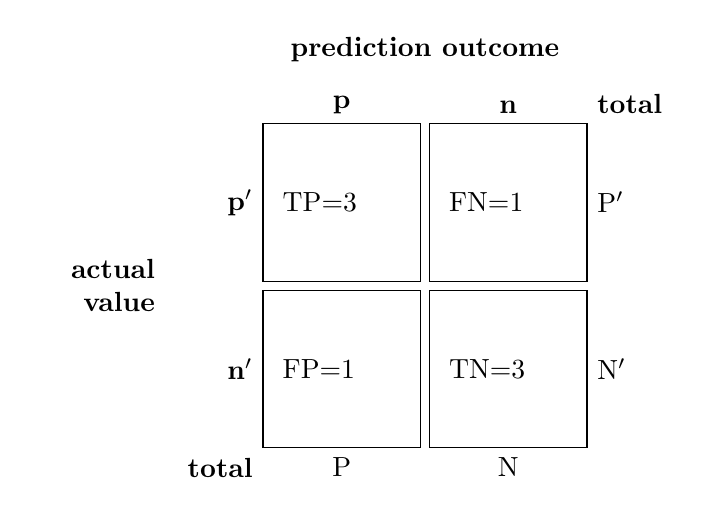
\begin{tikzpicture}[
box/.style={draw,rectangle,minimum size=2cm,text width=1.5cm,align=left}]
\matrix (conmat) [row sep=.1cm,column sep=.1cm] {
\node (tpos) [box,
    label=left:\( \mathbf{p'} \),
    label=above:\( \mathbf{p} \),
    ] {TP=3};
&
\node (fneg) [box,
    label=above:\textbf{n},
    label=above right:\textbf{total},
    label=right:\( \mathrm{P}' \)] {FN=1};
\\
\node (fpos) [box,
    label=left:\( \mathbf{n'} \),
    label=below left:\textbf{total},
    label=below:P] {FP=1};
&
\node (tneg) [box,
    label=right:\( \mathrm{N}' \),
    label=below:N] {TN=3};
\\
};
\node [left=.05cm of conmat,text width=1.5cm,align=right] {\textbf{actual \\ value}};
\node [above=.05cm of conmat] {\textbf{prediction outcome}};
\end{tikzpicture}
\\\\
\indent$F1_{C1}=\frac{2TP}{N+TP-TN}=\frac{6}{8+3-3}=\frac{3}{4}$\\\\
\indent(b)然后确定C2的混淆矩阵和F1度量\\\\
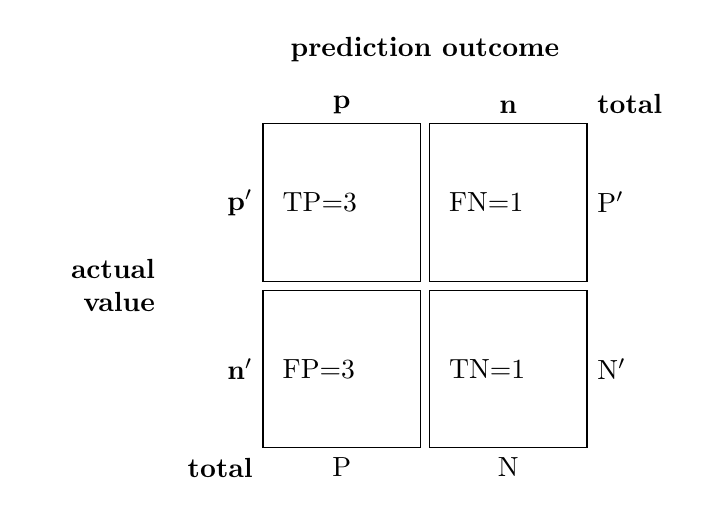
\begin{tikzpicture}[
box/.style={draw,rectangle,minimum size=2cm,text width=1.5cm,align=left}]
\matrix (conmat) [row sep=.1cm,column sep=.1cm] {
\node (tpos) [box,
    label=left:\( \mathbf{p'} \),
    label=above:\( \mathbf{p} \),
    ] {TP=3};
&
\node (fneg) [box,
    label=above:\textbf{n},
    label=above right:\textbf{total},
    label=right:\( \mathrm{P}' \)] {FN=1};
\\
\node (fpos) [box,
    label=left:\( \mathbf{n'} \),
    label=below left:\textbf{total},
    label=below:P] {FP=3};
&
\node (tneg) [box,
    label=right:\( \mathrm{N}' \),
    label=below:N] {TN=1};
\\
};
\node [left=.05cm of conmat,text width=1.5cm,align=right] {\textbf{actual \\ value}};
\node [above=.05cm of conmat] {\textbf{prediction outcome}};
\end{tikzpicture}
\\\\
\indent$F1_{C2}=\frac{2TP}{N+TP-TN}=\frac{6}{8+3-1}=\frac{3}{5}$\\\\
\indent从F1-Score来看依然是C1效果要好
\end{document}